%DIFF 1 new
\documentclass[letterpaper, 10 pt, conference]{ieeeconf}  % Comment this line out if you need a4paper
\IEEEoverridecommandlockouts                              % This command is only needed if
\overrideIEEEmargins                                      % Needed to meet printer requirements.

\usepackage{graphics}    % for pdf, bitmapped graphics files
\usepackage{times}       % assumes new font selection scheme installed
\usepackage{amsmath}     % assumes amsmath package installed
\usepackage{amssymb}     % assumes amsmath package installed
\usepackage{graphicx}
\usepackage{algorithm}
\usepackage[noend]{algpseudocode}
\usepackage[activate=alltext]{microtype}
\usepackage{rotating}


\usepackage{subcaption} % enables use multiple figures in a figure
\usepackage{tabu}     % provides advanced tables
\usepackage{booktabs} % enables reference bookstyle tables
\usepackage{xcolor}
\usepackage{import}
\usepackage{url}

% make captions look like original IEEE style
% table:  ieeeconf.cls:2017 \begin{center}{\footnotesize #1}\\{\footnotesize\scshape #2}\end{center}% figure: ieeeconf.cls:
% figure: ieeeconf.cls:2024 \setbox\@tempboxa\hbox{\footnotesize #1.~~ #2}%
\DeclareCaptionFont{ieeetable}{\footnotesize\scshape}
\DeclareCaptionLabelSeparator{ieeefigure}{.~~ }
\DeclareCaptionLabelSeparator{ieeetable}{\\[0.5em]}
\captionsetup[figure]{labelseparator=ieeefigure, font=footnotesize}
\captionsetup[table]{justification=centering, labelseparator=ieeetable, textfont=ieeetable, labelfont=footnotesize}
\captionsetup[subfigure]{font=footnotesize}
\captionsetup{subrefformat=parens}

%% Aligns the last page but causes errors on some machines (such as OSX), so don't use it for now.
\usepackage{flushend}

%% Style hacks to save space
%\setlength{\textfloatsep}{1.95em}
%\setlength{\dbltextfloatsep}{1.1em}
%\usepackage[font=small]{caption}

%% Key definitions for text elements. USE THEM
\def\secref#1{Sec.~\ref{#1}}
\def\figref#1{Fig.~\ref{#1}}
\def\tabref#1{Tab.~\ref{#1}}
\def\eqref#1{Eq.~(\ref{#1})}
\def\algref#1{Alg.~\ref{#1}}

%% Other useful macros
\newcommand\todo[1]{\textbf{[TODO: #1}]}
\newcommand\etal{\emph{et~al.}}


%% Some math definition
\def\argmax{\mathop{\rm argmax}}
\def\argmin{\mathop{\rm argmin}}
\newcommand{\bigO}[1]{$\mathcal{O}(#1)$}

%DIFF 2
%%%%%%%%%%%%%%%%%%%%%%%%%%%%%%%%%%%%%%%%%%%%%%%%%%%%%%%%%%%%%%%%%%%%%%%%%%%%%%%%

\title{\LARGE \bf Gradient-based Active Learning for Semantic Segmentation \\of Crop and Weed for Agricultural Robots}

\author{Rasha Sheikh \and Philipp Lottes \and Andres Milioto \and Cyrill Stachniss \and Maren Bennewitz \and Thomas Schultz% <-this % stops a space
  \thanks{All authors are with the University of
    Bonn, Germany. This work has partly been supported by the DFG-funded Cluster of Excellence EXC~2070 PhenoRob.}%
}

\begin{document}
\maketitle
\thispagestyle{empty} 
\pagestyle{empty}


%%%%%%%%%%%%%%%%%%%%%%%%%%%%%%%%%%%%%%%%%%%%%%%%%%%%%%%%%%%%%%%%%%%%%%%%%%%%%%%%
\begin{abstract}
Annotated datasets are essential for supervised learning. However, annotating
large datasets to  train deep neural networks that perform well is a tedious
and time-intensive task. This paper  addresses active learning in the context
of semantic segmentation with the goal of reducing the  human labeling effort.
Our target application is agricultural robotics and we focus on the task of
distinguishing between crop and weed plants from image data. A key challenge in this
application is the  transfer of an existing semantic segmentation CNN to a new
field. We propose a novel approach that, given a trained model on one field,
refines the network on a substantially different field  providing an effective
method of selecting samples to annotate for supporting the transfer. Our
method takes into account the influence of the so far unlabeled samples on the
weights of the network and  ranks and selects them accordingly for annotation.
We evaluated our approach on two challenging  datasets from the agricultural
robotics domain and show that we achieve a higher accuracy with a  smaller
number of samples compared to randomly selecting samples for annotation as well as
uncertainty-based  approaches to select examples for annotation. Thus, our
approach reduces the required human labeling  effort.

\end{abstract} 

%%%%%%%%%%%%%%%%%%%%%%%%%%%%%%%%%%%%%%%%%%%%%%%%%%%%%%%%%%%%%%%%%%%%%%%%%%%%%%%%
\section{INTRODUCTION}
\label{sec:intro}

The ability to  interpret the scene in front of a robot is key for
intelligent behavior in several applications. For example, precision farming
robots need to know which type of plant they perceive or autonomous cars need to
know  which object in their surroundings is a car, a pedestrian, or a
cyclist. These  classification or semantic segmentation tasks are typically
tackled using  convolutional neural networks~(CNNs) operating on  image data.
In order to perform  well, neural networks need to be trained with
appropriately annotated datasets.

The performance of most supervised learning approaches and especially deep
learning  systems is related to the quality and quantity of training data.
Annotated training data, however, has a high cost as often a larger number of
labeled training data is  required.  In this work, we focus on optimizing the
training set generation for  semantic segmentation of image data obtained
from a mobile robot. Semantic segmentation refers to the task of computing a
pixel-wise  labeling of the images. More concretely, we address the
agricultural robotics  application in which robots should perform automated
weed control. For the semantic  segmentation, this means that we need to
compute the semantic label ``crop'', ``weed'',  or ``misc'' for every pixel in
the image. This task is particularly challenging  as the field conditions
often change substantially between years, regions, weather, and  soil
conditions. Thus, one often tries to adapt and refine existing semantic
segmentation systems to new field conditions through annotated data from the
new field. As these new annotation need to be executed at the end-users site,
one is interested in keeping this effort as low as possible. Thus, this
problem is a perfect domain for active  learning approaches trying to reduce
the required amount of data to be annotated.

Given annotated data on one agricultural field and a network that was trained
on it, we address the problem of transferring this knowledge to new fields with
minimum effort.  Datasets from different fields reveal different crop and weed
statistics. They almost  always differ by soil type, weather condition, or
various small objects that can be found  on the ground, such as stones, dried
vegetation, or marks from agricultural machines,  i.e., patterns that are
neither crop nor weed. Additionally, the robot can acquire  images of plants
at a certain growth stage in one field, while the growth state on the  target
field is different. Lastly, artifacts such as contrast changes can be found in
the camera images captured from the various locations.  These conditions make
it difficult to simply reuse a previously trained network from one  field and
infer the labels on another~\cite{lottes2018ral,lottes2017iros}. Thus, 
the network has to be
re-trained on  annotated images taken in the new field. We propose an
active learning  approach to select samples that the network will most benefit
from and will generalize  to the rest of the unlabeled data while minimizing
the effort of annotating images.

The main contribution of this work is an active learning approach that
intelligently picks images taken under the new conditions based on the effect
these training samples will have on the weight gradients of the CNN. Our
strategy is based  on the observation that given a trained model and unseen
samples from  a different domain, the samples that the network performs most
poorly on, especially at the  beginning, will have the largest weight
gradients and consequently the largest impact on the  weights. This strategy might appear to be circular, since computing gradients already requires class labels at a stage where are still selecting images for labeling.  We circumvent this by using pseudo ground truth that we obtain with very weakly supervised segmentation. Our approach
selects samples in batches, each time refining the network, then computing a
new  ranking of the unlabeled data. The best samples are then selected and the
network is re-trained. To compute the real gradients, corresponding ground
truth data is needed. Thus, in our approach, we approximate the ground truth as the result of unsupervised segmentation to estimate the gradient.  We
evaluated our framework on  agricultural datasets~\cite{chebrolu2017agricultural} 
with different characteristics.  Our results indicate that our method produces a
higher accuracy on the datasets with a fewer  number of samples compared to
random sampling for annotation as well as uncertainty-based approaches.



%%%%%%%%%%%%%%%%%%%%%%%%%%%%%%%%%%%%%%%%%%%%%%%%%%%%%%%%%%%%%%%%%%%%%%%%%%%%%%%%
\section{RELATED WORK}
\label{sec:related}

Several works focusing on the elimination or reduction of herbicide use
through the incorporation of autonomous ground robots in our crop fields have
been introduced to the community in the last years~\cite{ducket2018arxiv, liebisch2016wslw, mccool2018ral}.
A key component of each of these unmanned platforms is a core perception system that
has the ability to accurately distinguish value crops from weeds in order to effectively
and selectively apply the desired individual treatment~\cite{ lottes2018iros, mccool2017ral,milioto2017uavg,milioto2018real, sa2018rs}.
These systems allow autonomous robots to perform actuation in the fields without human supervision, treating each plant individually.
All of the works referenced, however, are based on supervised learning approaches which take large amounts of pixel-accurate hand-labeled images for training. 
Accordingly, one of the main bottlenecks of these visual processing pipelines is the amount of expensive labeled training data required to deploy them in real agricultural fields, which often limits their applicability.

In order to tackle this data starvation problem, we propose an active learning based solution. Numerous works on general active learning have been presented in the community~\cite{settles2009active,guyon2011results,holub2008entropy}. Recently, the research topic of using active learning in combination with deep learning has received attention. We focus in this section on the different approaches that explored active learning within a deep learning framework.

Settles~\cite{zhou2017fine} defines measures of entropy and diversity to select new samples for annotation. The entropy of a patch is calculated based on the classification uncertainty of the network, whereas the diversity is computed using the Kullback Leibler divergence of different patches within the same sample candidate. A pre-trained network is then refined using the samples with the highest entropy and diversity.

Yang~\etal~\cite{yang2017suggestive} select samples that the network is uncertain of and that are representative of other images in the dataset. The uncertainty is measured by bootstrapping, where multiple fully convolutional networks (FCNs) are trained, and the variance among  these trained models is used to estimate the uncertainty. In order to choose samples that are highly similar to others in the training set, features are extracted from the encoding part of the network, and the cosine similarity between pairs of images is calculated. 

Dutt Jain~\etal~\cite{dutt2016active} create foreground masks in an iterative manner. Samples that are deemed most valuable for annotation are selected. Their ground truth annotation is then propagated to new samples and the process is repeated. To pick samples for which human annotation will propagate well, the authors build a Markov Random Field (MRF) joint segmentation graph. The graph is then used to find samples that have the largest influence, diversity and uncertainty. The influence and diversity are computed using the cosine-similarity of different images features, while the uncertainty is estimated using a regressor that quantifies the quality of a prediction. 

Gal~\etal~\cite{gal2017deep} evaluate different acquisition functions. An active learning system would use such an acquisition function to choose the best next sample to annotate. These functions include maximizing the predictive entropy of a model given the training set and a new sample, and closely related to that is the variation ratio measure. Another function maximizes the mutual information between predictions and the model posterior. These different measures are compared using a Bayesian Convolutional Neural Network that has a prior probability distribution over the model parameters.  

Uncertainty estimation for active learning can be performed using Monte-Carlo dropout as in~\cite{gal2017deep} or with an ensemble of deep networks. These uncertainties can then be used in the different acquisition functions described earlier. Beluch~\etal~\cite{beluch2018power} compare both of these approaches on different datasets. They found that an ensemble of deep classifiers has a superior performance even with a smaller number of models. They conclude that Monte-Carlo dropout approaches suffer from a lower diversity and a smaller model capacity.

Sener~\etal~\cite{sener2017geometric} assert based on the experiments they performed that uncertainty based approaches are not effective for active learning with CNNs. They hypothesize that this is not due to the inaccurate estimate of uncertainty by the network, rather by the ineffectiveness of uncertainty based approaches to cover the space of image features. They instead propose to choose samples such that the largest distance between a new sample and its closest neighbor in the selected subset is minimized.

Wang~\etal~\cite{wang2017cost} select two sets of samples for annotation that can then be used by the network to refine the model. The first set consists of samples that the network is uncertain about. These include samples with the lowest softmax confidence values, samples with the highest entropy, and lastly samples with a small margin of probability difference between the most probable class and the second most probable class. This first set is then presented to a human for annotation. The second set consists of samples that the network is highly certain about, these are assigned their predicted classes as pseudo labels and added to the set of training samples without asking a human to annotate them.

The Expected Model Output Change Principle (EMOC) developed by Freytag~\etal~\cite{freytag2014selecting} tries to avoid selecting samples that are redundant and K{\"a}ding~\etal~\cite{kading2016active} follow this approach with deep neural networks. This principle measures how a model would perform with and without the candidate sample. Given that the labels are unknown, a marginalization over the possible labels is needed. This marginalization however can be expensive when having a large number of classes, so the authors use maximum a-posteriori approximation instead and use the class with the highest probability prediction.

In the context of self-learning, Zhang~\etal~\cite{zhang2018self} use labels obtained with K-means graph cuts as ground truth for their network. The predictions produced by the model are then used as the target labels for the next iteration of the process.  

Different to these works, we experiment with approaches that directly measure how annotated samples can affect the gradients. We use labels obtained with very weak supervision as pseudo ground truth and compute the gradients w.r.t the weights. We then refine a pre-trained network with the newly annotated samples in an iterative manner. 




\section{Segmentation Framework} \label{sec:approach}


    \begin{figure*}
    \centering
    \includegraphics[scale=0.9]{pics/output_system_overview.pdf}
   		\caption{Overview figure of our system. We first perform very weakly supervised segmentation to obtain pseudo ground truth. Given the labels and different measures produced by the network, we rank the unlabeled samples and pick them accordingly for annotation. These are then used to refine the network.}
		\label{fig:overview}    		
%    \vspace{1em}
   \end{figure*}


We use Bonnet~\cite{milioto2018bonnet} to train a model on the Bonn sugar beet dataset~\cite{chebrolu2017agricultural}. We then refine the trained model on other datasets by incrementally selecting batches of samples. The datasets differ in their crop/weed statistics and the images acquired with the cameras also differ in their illumination. Therefore, simply running the trained model to segment the vegetation in other fields does not work. We briefly first describe the architecture of the network used, then present different methods to select samples for refinement that we experimented with.


Bonnet is an open-source deep network framework developed by \cite{milioto2018bonnet}. It was designed with efficiency in mind so that it is able to run at 20 Hz. The network is based on SegNet \cite{badrinarayanan2017segnet} and ENet \cite{paszke2016enet}. It has an encoder-decoder structure with a total of 25 [5x5] convolutional layers. It uses batch normalization, residual connections, and ReLU as the non-linearity layer. 

To speed up prediction, the authors replace the [5x5] conventional convolutional layer with a mix of [1x1] convolutions and separable [1x5] and [5x1] convolutions. Additionally, instead of using the relatively more expensive transposed convolutions in the decoder, unpooling is done using the respective pooling indices in the encoder part.

As input to our network we only use the RGB channels.


%Network was designed with efficiency in mind.
%has an encoder decoder structure
%runs at 20 Hz
%
%As input we only used the RGB images
%
%used batch normalization, ReLU as non linearity
%
%residual connections
%
%mix of 1x1 convolutions and separable convolutions to increase the speed
%
%unpooling in the decoder is done using the respective pooling indices in the encoder part. instead of using the relatively more expensive transposed convolutions
%
%25 convolutional layers.


\section{Effective Sample Selection}

We experimented with different approaches to select samples. The baseline is randomly selecting samples for annotation in batches of 10. The other approaches include selecting samples driven by the uncertainty of the network, the training loss, and the weight gradients of the network.   


\subsection{Uncertainty}

To infer the pixel-wise semantic segmentation of a new image, the network computes softmax probabilities in its last layer. The probabilities can serve as a guide as to which samples the network is most uncertain of. For every image passed through the network, we compute the following measure of the prediction confidence:
\begin{align}
u(\bold{x}) &= \frac{1}{N} \sum_{i=1}^N \max_c p(c|x_i),
\end{align}  

where $x_i$ is pixel $i$ in the image and $c$ is the predicted class.

We then sort the images based on the computed uncertainty measure and pick the images accordingly to refine the network on a new dataset. The images are selected on a log-space scale, rather than selecting those with the highest uncertainty, as we found out that the network learns better when presented with diverse samples. The log-space approach is used in the following methods as well.

\subsection{Loss} \label{sec:loss}

The loss of the network is an indication of the segmentation error. Given that training neural networks with backpropagation is driven by the loss, it also provides a useful cue as to which samples the network will most benefit from. We compute the loss based on a pseudo-ground truth, consisting of a foreground-background segmentation that we achieve using k-means clustering on the RGB channels.

Initially, we use k-means to determine 20 cluster representatives from 10 randomly selected images. After viewing a single image that contains all 20 clusters, a human annotator chooses which clusters represent vegetation. In our experiments, it was enough to select two clusters. In accordance with previously used terminology \cite{zhang2018self}, we refer to this step as being very weakly supervised, since it only involves inspecting a single image. 

Pseudo ground truth is generated for all unlabeled images by assigning pixels to the selected clusters, and the loss is computed with respect to it. The images are sorted based on this loss and again chosen on a log-space scale. We note that the pseudo ground truth is only used to compute the loss but the network weights remain unchanged. They are only later updated with the manual annotations of the selected samples.


\subsection{Norm of Gradients} \label{sec:grad_norm}

For this approach and the following one, we pick those samples for annotation that might have the largest impact on the network weights. The norm of the network gradients is a measure that is indicative of which samples will affect the weights more than others. As in the previous approach, we use labels from very weakly supervised segmentation as pseudo ground truth. We run the network on the training images for one epoch and compute the gradients. Again we note that this step is only used to compute the gradients but we don't change the network weights. Once we have the gradients, we compute the $L_2$ norm of those in the last two layers of the network (the classifier layer and the one immediately before it).
\begin{align}
n_g(\bold{x}) &=  \left\lVert \nabla_{w_f} \mathcal{L}(\bold{x}) \right\rVert,
\end{align}  
where $w_f$ are the weights of the final layer.

The images are sorted based on this measure and we pick samples on a log-space scale afterwards.

\subsection{Gradient Projection} \label{sec:grad_proj}

The log-space in the previous approaches was used to ensure there is enough diversity among the samples so that the network does not overfit on them and can generalize to unseen data. Here we use a different method that relies on the space spanned by the gradients where we project onto the orthogonal complement of the gradients of the selected samples. For every sample picked we project the gradients of all remaining samples onto the selected sample gradient. We then subtract the projected gradient from the original gradients. The residual we are left with indicates which samples have the strongest remaining effect on the weights after accounting for the already selected samples. This can be formulated as:
\begin{align}
n_p(\bold{x}) &=  \left\lVert \bold{g_x} - \sum_{i=1}^S \frac{\left\langle \bold{g_i}, \bold{g_x} \right\rangle}{\left\langle \bold{g_i}, \bold{g_i} \right\rangle} \bold{g_i} \right\rVert,
\end{align}
where $\bold{g_i}$ is the gradient of the $i$th out of $S$ previously selected samples, and $\bold{g_x}$ is the gradient of the current sample.

We select samples one by one, each time sorting them according to this measure and choosing the one with the highest norm of the residual. To pick the first sample, we choose that with the highest norm of the gradient.



%%%%%%%%%%%%%%%%%%%%%%%%%%%%%%%%%%%%%%%%%%%%%%%%%%%%%%%%%%%%%%%%%%%%%%%%%%%%%%%%
\section{EXPERIMENTAL EVALUATION}
\label{sec:exp}


We show in this section the effectiveness of the approaches we designed for active learning, where samples are selected using the different methods and the performance is tested on different datasets. 


\subsection{Datasets}

The datasets we used were acquired with a Bosch Deepfield Robotics BoniRob UGV in three different fields: Bonn and Stuttgart in Germany, and Zurich in Switzerland. The datasets have weed and crop plants at different stages of growth. Figure \ref{fig:datasets_images} shows sample images from the different datasets. The images vary in their illumination, soil type, and class statistics, hence the need for transfer learning. The images have been annotated into three classes: soil, weed and crop. The Bonn dataset is partly publicly available \cite{chebrolu2017agricultural}. Table \ref{tab:datasets_stats} shows the number of images in each dataset and the ratio of foreground pixels. It can be clearly seen that there is a high imbalance of classes in the data.



    \begin{table}
        \centering
        \caption{Datasets Statistics of Crop and Weed Plants}
        \begin{tabular}{@{}lccccc@{}} 
            \toprule
              & Bonn & Stuttgart & Zurich \\ 
            \midrule 
    		  Images  & 8230 & 2584 & 2577 \\ \addlinespace
    		  Crop pixels & 2.0\% & 1.5\% & 0.4\%  \\ \addlinespace
    		  Weed pixels & 0.3\% & 0.7\% & 0.1\%  \\    
            \bottomrule
        \end{tabular}
        \label{tab:datasets_stats}
    %       \vspace{10em}
    \end{table}
    
    
    
    \begin{figure}
    \centering
     \begin{subfigure}[b]{0.49\linewidth}
    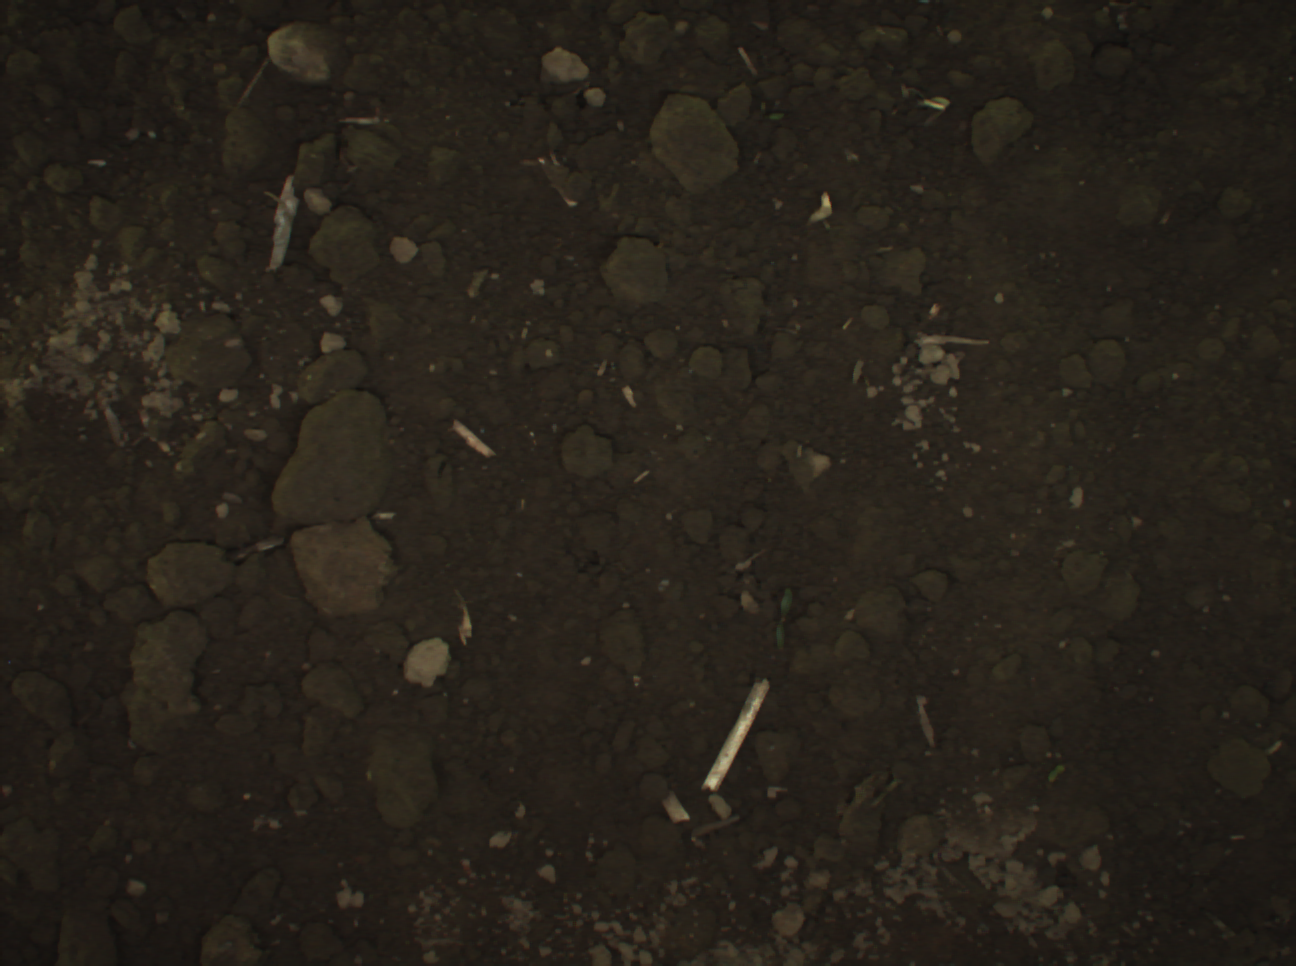
\includegraphics[width=\linewidth]{pics/bonn/images/bonirob_2016-04-28-12-20-29_6_frame217.png}
   		\caption{}
		\label{bonn_img}    		
   \end{subfigure}
        \begin{subfigure}[b]{0.49\linewidth}
    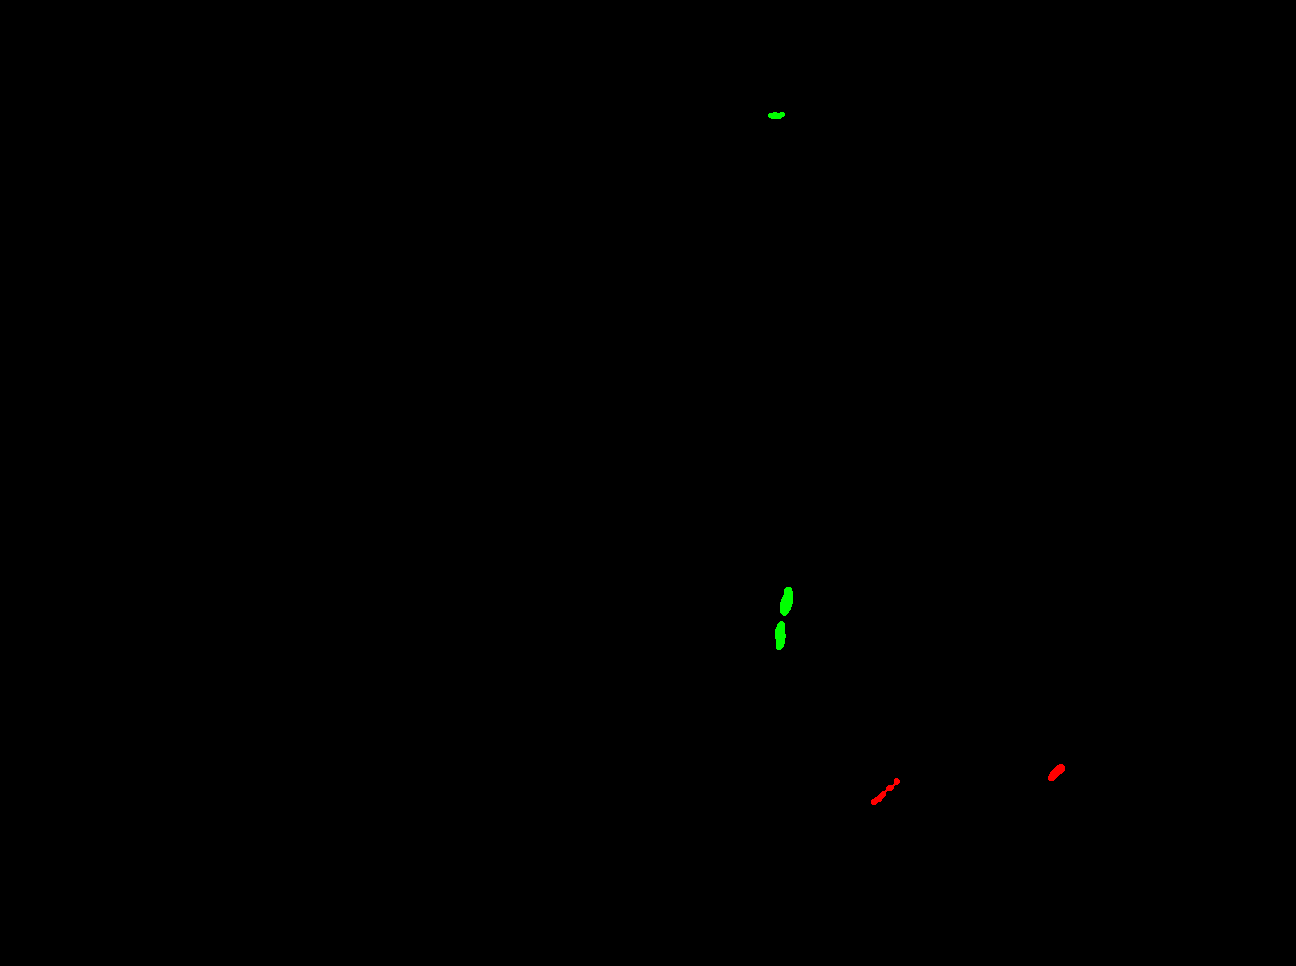
\includegraphics[width=\linewidth]{pics/bonn/annotations/bonirob_2016-04-28-12-20-29_6_frame217.png}
   		\caption{}
		\label{bonn_lbl}    		
   \end{subfigure}
        \begin{subfigure}[b]{0.49\linewidth}
    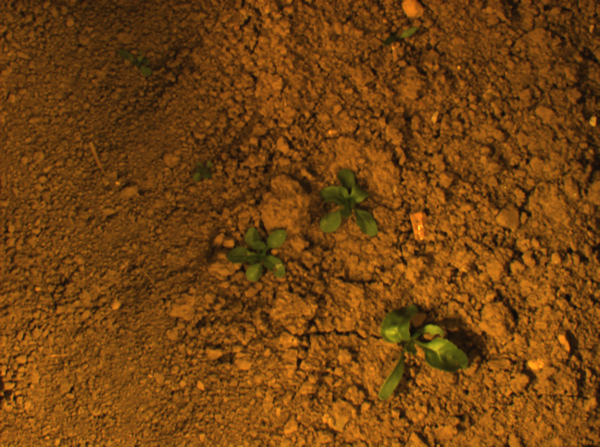
\includegraphics[width=\linewidth]{pics/stuttgart/images/masks_8mm_fromImages_frame479.png}
   		\caption{}
		\label{stuttgart_img}    		
   \end{subfigure}
        \begin{subfigure}[b]{0.49\linewidth}
    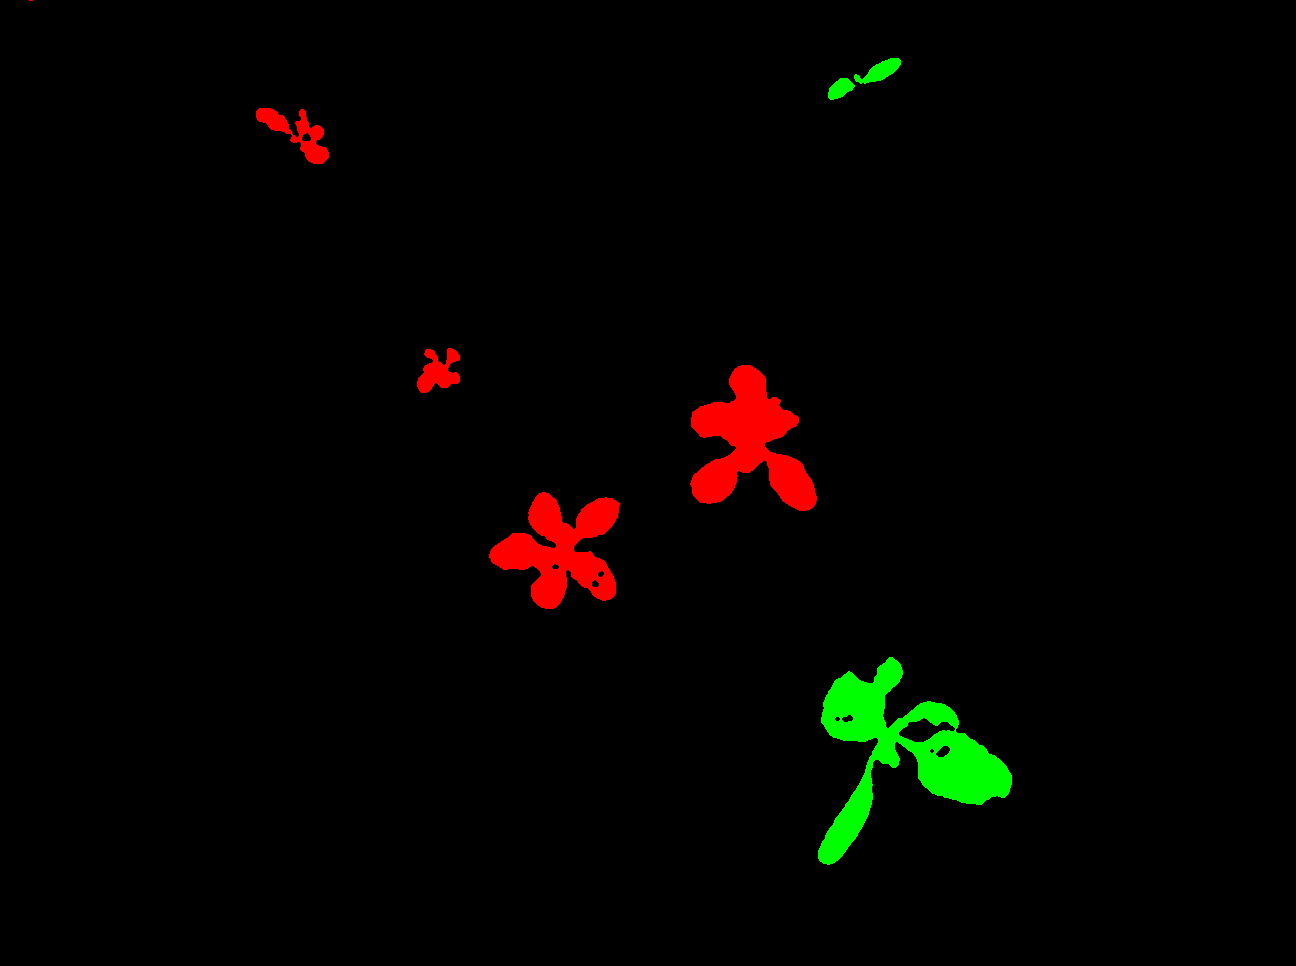
\includegraphics[width=\linewidth]{pics/stuttgart/annotations/masks_8mm_fromImages_frame479_GroundTruth_iMap.png}
   		\caption{}
		\label{stuttgart_lbl}    		
   \end{subfigure}
        \begin{subfigure}[b]{0.49\linewidth}
    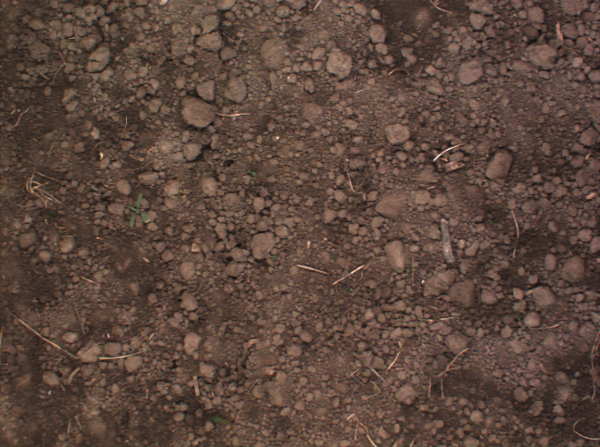
\includegraphics[width=\linewidth]{pics/zurich/images/bonirob_2016-10-13-09-03-00_0_frame66.png}
   		\caption{}
		\label{zurich_img}    		
   \end{subfigure}
        \begin{subfigure}[b]{0.49\linewidth}
    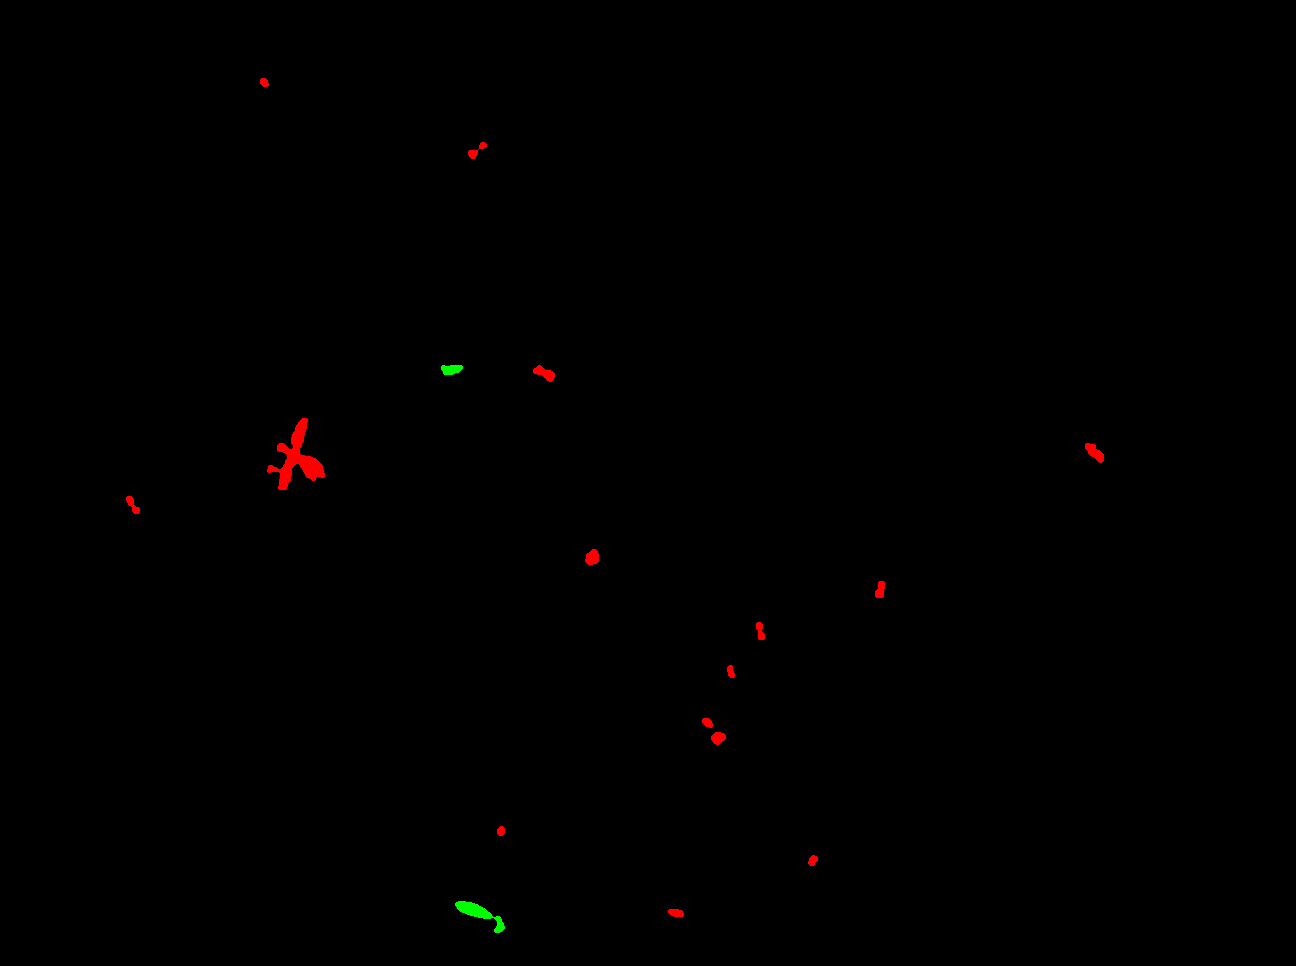
\includegraphics[width=\linewidth]{pics/zurich/annotations/bonirob_2016-10-13-09-03-00_0_frame66.png}
   		\caption{}
		\label{zurich_lbl}    		
   \end{subfigure}
    \caption{Sample images from the Bonn, Stuttgart, and Zurich datasets in the first, second, and third row respectively. The first column shows the RGB images and the second column shows their annotations. Green denotes crop while red denoted weed.}
    \label{fig:datasets_images}
\end{figure}



    
    \begin{figure}
    \centering
     \begin{subfigure}[b]{0.31\linewidth}
    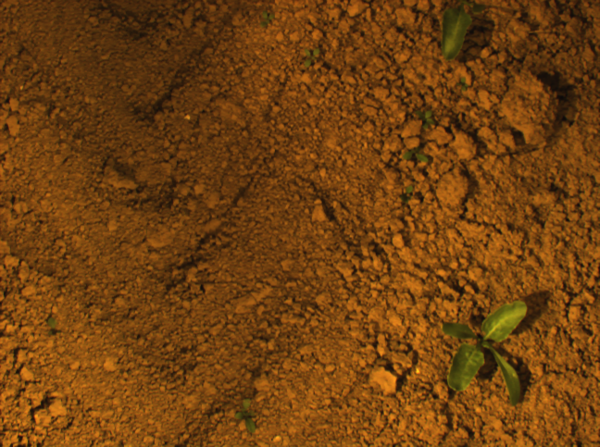
\includegraphics[width=\linewidth]{pics/unsupervised/img_masks_8mm_fromImages_frame256.png}
   		\caption{input}
		\label{unsup_img}    		
   \end{subfigure}
        \begin{subfigure}[b]{0.31\linewidth}
    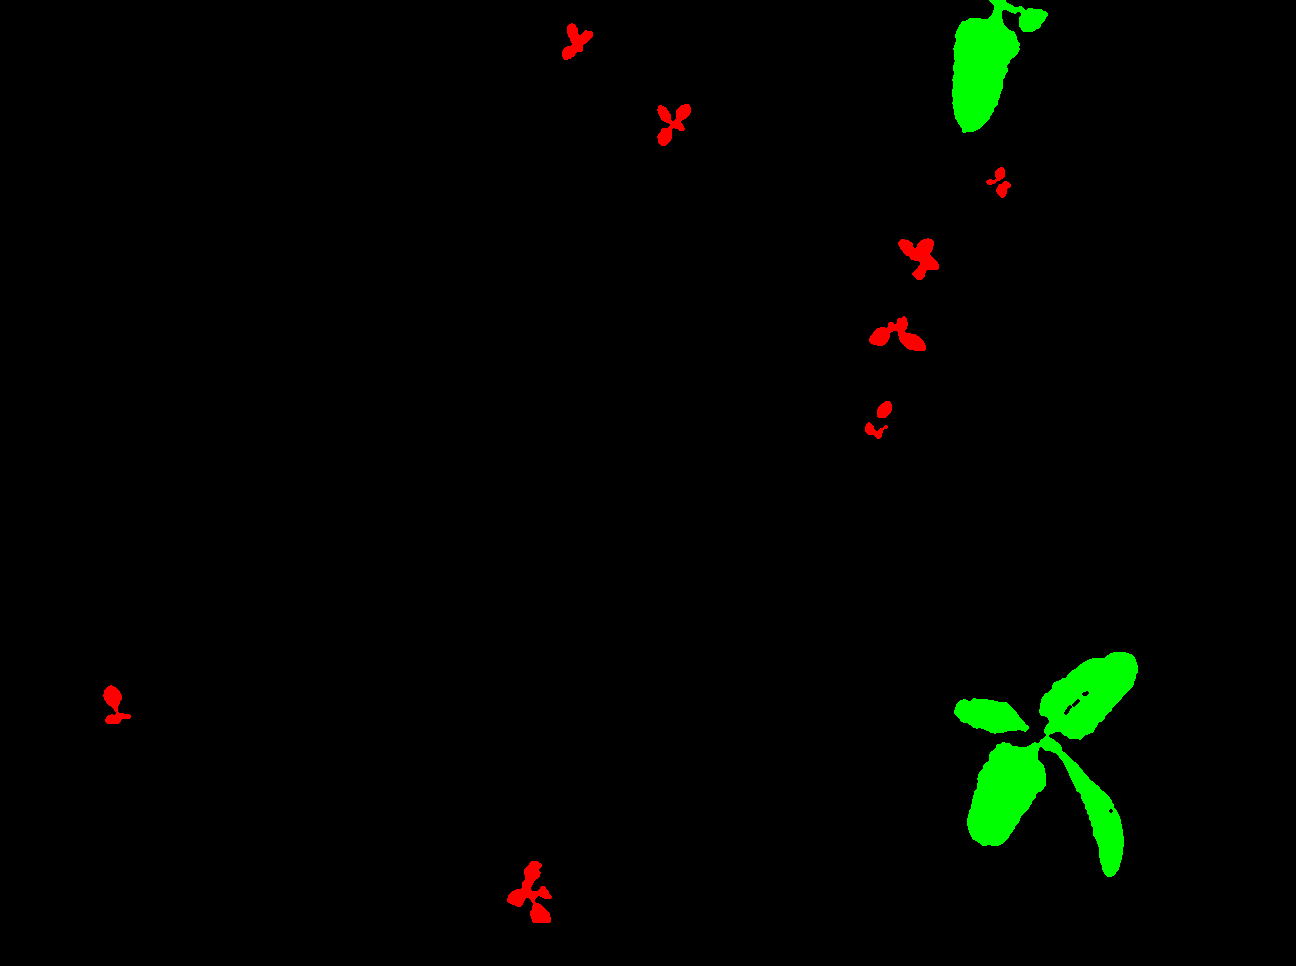
\includegraphics[width=\linewidth]{pics/unsupervised/gt_masks_8mm_fromImages_frame256_GroundTruth_iMap.png}
   		\caption{ground truth}
		\label{unsup_gt}    		
   \end{subfigure}
      \begin{subfigure}[b]{0.31\linewidth}
    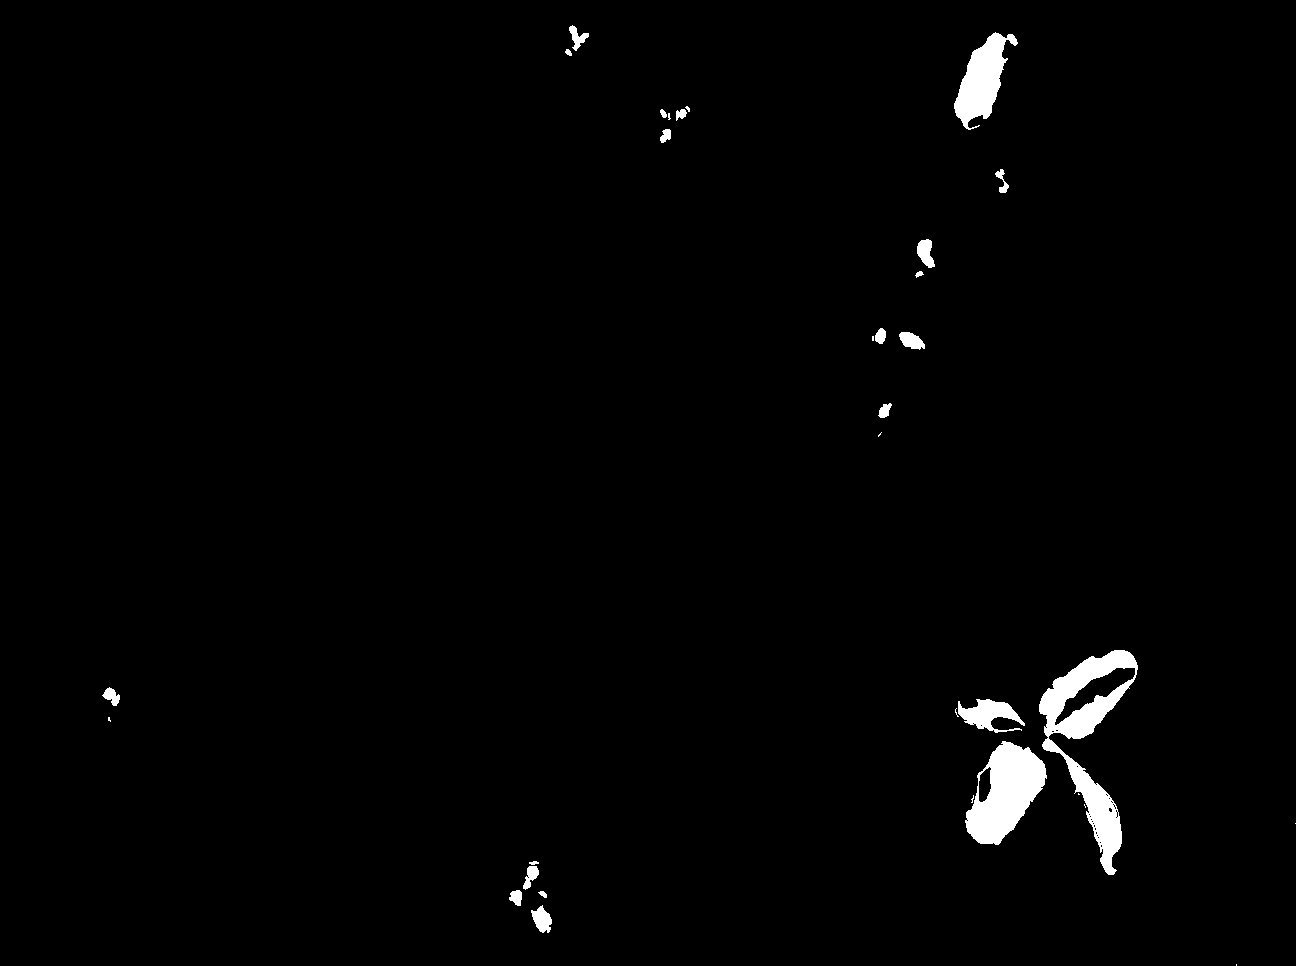
\includegraphics[width=\linewidth]{pics/unsupervised/lbl_masks_8mm_fromImages_frame256.png}
   		\caption{segmentation mask}
		\label{unsup_lbl}    		
   \end{subfigure}
    \caption{Foreground segmentation of vegetation. Note that only a rough segmentation is enough for our approach.}
    \label{fig:unsupervised_foreground}
\end{figure}


\subsection{Experiment Setup}

We evaluate our different approaches by first training a network on the Bonn dataset then refining it on the Stuttgart and Zurich datasets. To refine the network we pick unlabeled samples in batches of 10 using one of the methods described in Section \ref{sec:approach}. Once they are annotated, they are presented to the network. We repeat this process iteratively, each time refining the network on all of the newly annotated samples. 

For the methods presented in sections \ref{sec:loss}, \ref{sec:grad_norm}, and \ref{sec:grad_proj}, we first obtain foreground masks with very weak supervision. Figure  \ref{fig:unsupervised_foreground} shows an image, its ground truth and the foreground segmentation provided by clustering. It is an important finding from our experiments that a rough segmentation is sufficient for the purpose of selecting images for annotation. This makes our proposed gradient-based approach feasible in practice.

We follow the approach of \cite{milioto2018real} and split the new dataset into three sets: 40\% for training, 10\% for validation, and 50\% for testing. The samples are picked from the training set. All experiments were conducted on four Titan X GPUs.  

\subsection{Results}


    \begin{figure}
    \centering
    \vspace{-1em}
    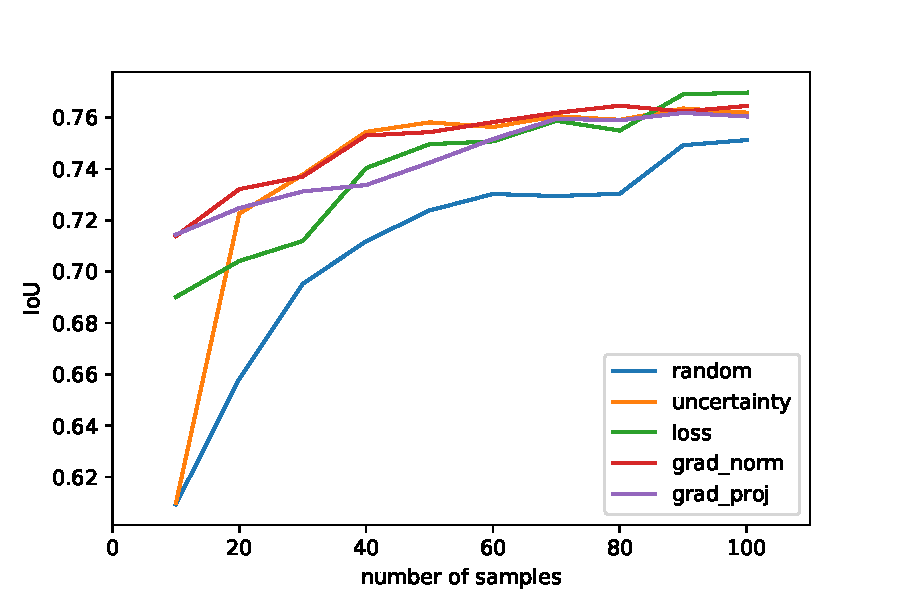
\includegraphics[width=\linewidth]{pics/pw_iou_stuttgart.pdf}
   		\caption{Pixel-wise mean IoU on the Stuttgart dataset.}
		\label{fig:iou_stuttgart}    		
%    \vspace{1em}
   \end{figure}
   
    \begin{figure}
    \centering
    \vspace{-1em}
    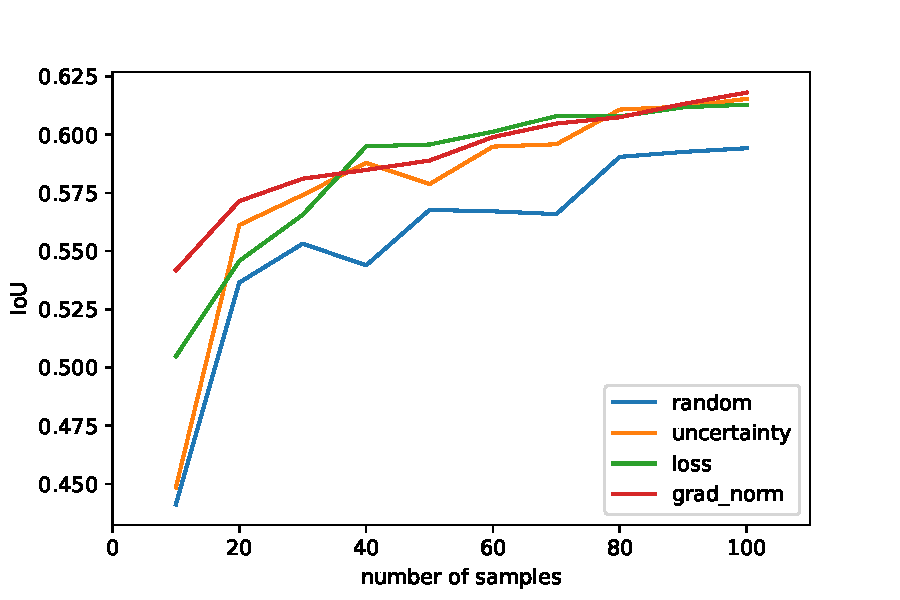
\includegraphics[width=\linewidth]{pics/pw_iou_zurich.pdf}
   		\caption{Pixel-wise mean IoU on the Zurich dataset.}
		\label{fig:iou_zurich}    		
 %   \vspace{1em}
   \end{figure}
   

Figures \ref{fig:iou_stuttgart} and \ref{fig:iou_zurich} show the pixel-wise mean intersection over union (mIoU) on the Stuttgart and Zurich datasets when selecting samples for annotation with different methods. It can be seen from the plots that methods that take into account the impact of the samples on the weights lead to better generalization to the rest of the unseen data, even when presented with a small number of annotated images. In particular, ranking the samples based on the norm of the gradients results in higher mIoU on both datasets.

To further quantify the performance of our approach, we use the object-wise metric defined by \cite{milioto2018real}, where the accuracy is measured for objects larger than 50 pixels. Since the target application is weeding with agricultural robotics, this metric is more directly useful than pixel-wise performance.  


Tables \ref{tab:stuttgart} and \ref{tab:zurich} show how our approach performs on the Stuttgart and Zurich datasets. Each row shows the mean accuracy when selecting $n$ samples with different methods. The baseline is random sampling shown in the first column.

%As can be seen from the result,

A few observations can be made: the effect of the sampling method is more pronounced when only a few images are selected. Again, it can be seen that methods measuring the influence of the samples on the weighs perform better. For instance, training a model with 20 samples picked with the gradient norm method produces accuracies that can only be achieved when picking 60 samples with the random method, lowering the annotation effort considerably.

As the model is trained on more and more samples, the accuracy plateaus as is expected and the variation between the different methods decreases. It can be noted however that random sampling has a lower performance even with a greater number of images.

The gradient norm method shows a consistent improvement over other methods for different number of samples and across the two datasets, confirming that samples that might have a larger influence on the weights are more valuable for annotation, as the network can benefit more from them.

Projecting out the gradients iteratively seems to be a promising method. For small number of images, it performs best but then the improvement afterwards is not as noticeable. Investigating the images that are being chosen in the fourth row and beyond for this method, we hypothesize that although these images will force the network weights to change in orthogonal directions, they might not be representative of a larger subset of images in the dataset. We plan to investigate this further in the future. 



 
 %  \begin{subfigure}[b]{0.49\linewidth}

    

   
   
%          \begin{table}
%        \centering
%        \caption{asdasd}
%        \begin{tabular}{@{}lcccccc@{}} 
%            \toprule
%              Approach & Weed & Crop & Weed & Crop & Weed & Crop \\ 
%            \midrule 
%    		  Random & 2.0 & 1.5 & 0.4095 & 0.7278 & 0.4851 & 0.6946  \\ \addlinespace
%    		  Uncertainty & 2.0 & 1.5 & 0.5580 & 0.6646 & 0.2711 & 0.8880  \\ \addlinespace
%    		  Loss & 2.0 & 1.5 & 0.5331 & 0.8025 & 0.6179 & 0.8112  \\ \addlinespace
%    		  Gradient Norm & 2.0 & 1.5 & 0.5970 & 0.8259 & 0.6136 & 0.8402  \\ \addlinespace
%    		  Gradient Projection & 2.0 & 1.5 & 0. & 0. & 0. & 0.  \\ 
%            \bottomrule
%        \end{tabular}
%        \label{tab:Pixelwise}
%    %       \vspace{10em}
%    \end{table}
%   
   
   
A more detailed breakdown of the methods performance is shown in tables \ref{tab:pixel_wise_10_stuttgart} and \ref{tab:object_wise_10_stuttgart}. Table \ref{tab:pixel_wise_10_stuttgart} shows the pixel-wise precision and recall on the Stuttgart dataset after selecting the first 10 samples. Both methods, Gradient Norm and Gradient Projection have a high recall and precision of the crop class without degrading those of the weed class. The object-wise performance in Table \ref{tab:object_wise_10_stuttgart} further illustrates the effectiveness of these methods. Gradient Norm and Gradient Projection produce high precision and recall for both classes. The Uncertainty-based method, on the other hand, shows a large imbalance of performance on the two classes.
   
   
   
       \begin{table}
        \centering
        \caption{Pixel-wise precision and recall on the Stuttgart dataset after selecting the first 10 samples}
        \begin{tabular}{@{}lcccc@{}} 
            \toprule
            & \multicolumn{2}{c}{Precision} & \multicolumn{2}{c}{Recall}\\ 
           \cmidrule{2-5} 
               & Weed & Crop & Weed & Crop \\ 
            \midrule 
    		  Random & \textit{0.4095} & 0.7278 & 0.4851 & \textit{0.6946}  \\ \addlinespace
    		  Uncertainty & 0.5580 & \textit{0.6646} & \textit{0.2711} & \textbf{0.8880}  \\ \addlinespace
    		  Loss & 0.5331 & 0.8025 & 0.6179 & 0.8112  \\ \addlinespace
    		  Gradient Norm & \textbf{0.5970} & 0.8259 & 0.6136 & 0.8402  \\ \addlinespace
    		  Gradient Projection & 0.5745 & \textbf{0.8365} & \textbf{0.6564} & 0.8212  \\ 
            \bottomrule
        \end{tabular}
        \label{tab:pixel_wise_10_stuttgart}
    %       \vspace{10em}
    \end{table}
   
   
   
   
          \begin{table}
        \centering
        \caption{Object-wise precision and recall on the Stuttgart dataset after selecting the first 10 samples}
        \begin{tabular}{@{}lcccc@{}} 
            \toprule
            & \multicolumn{2}{c}{Precision} & \multicolumn{2}{c}{Recall}\\ 
           \cmidrule{2-5} 
               & Weed & Crop & Weed & Crop \\ 
            \midrule 
    		  Random & \textit{0.8723} & 0.5740 & 0.6587 & 0.6474  \\ \addlinespace
    		  Uncertainty & \textbf{0.9476} & \textit{0.4586} & \textit{0.4919} & \textbf{0.8854}  \\ \addlinespace
    		  Loss & 0.9005 & 0.6898 & 0.7811 & 0.7351  \\ \addlinespace
    		  Gradient Norm & 0.9090 & \textbf{0.7390} & 0.7970 & 0.7536  \\ \addlinespace
    		  Gradient Projection & 0.9030 & 0.7308 & \textbf{0.8289} & 0.7375  \\ 
            \bottomrule
        \end{tabular}
        \label{tab:object_wise_10_stuttgart}
    %       \vspace{10em}
    \end{table}
   
   
  To analyze the samples picked by the gradient based approach, we plot the t-distributed Stochastic Neighbor Embedding (t-SNE) of the gradients in Figure \ref{fig:tsne}. Each circle in the plot denotes the 2-D embedding of the gradients of a single image before picking the first 10 samples. Red circles in the figure denote images selected by the Gradient Norm method. Points in the bottom left have a large norm of gradients, while the point in the upper left has the lowest norm of the gradient. Given the log-spacing of the selected samples, it can be seen that it more densely selects images that the network finds difficult, and the other selected points are more spread out. For future work, we plan to investigate how this embedding can be further exploited to pick the best samples.
   
       \begin{figure}
    \vspace{-1em} 
    \centering
    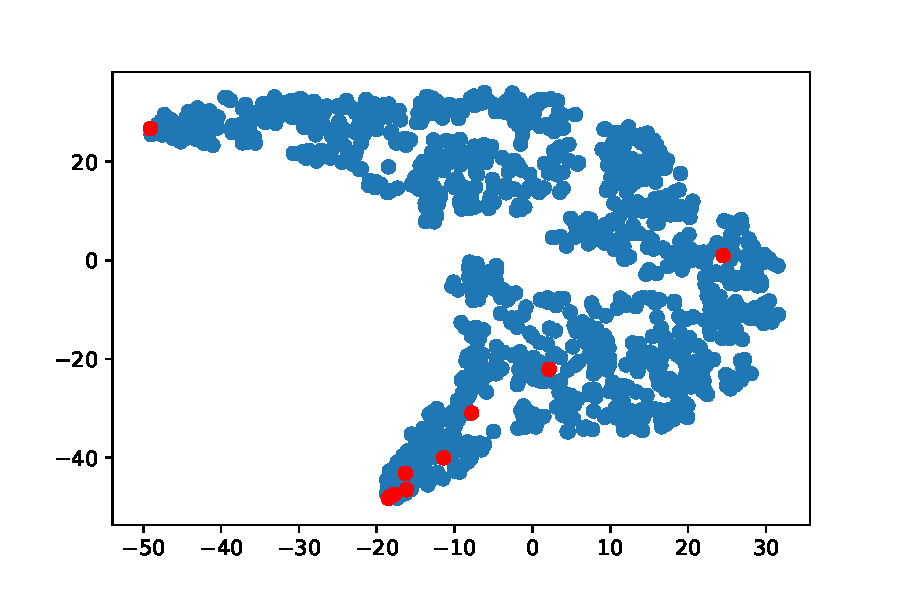
\includegraphics[width=\linewidth]{pics/tsne_grad_norm.pdf}
   		\caption{t-SNE of the images gradients on the Stuttgart dataset. The first 10 samples selected by the gradient norm method are shown in red.}
		\label{fig:tsne}    		
 %   \vspace{1em}
   \end{figure}







    \begin{table}
        \centering
        \caption{Object-wise Performance on the Stuttgart dataset. Each row shows the performance after selecting 10 samples with the different methods and refining the network.}
        \begin{tabular}{@{}cccccc@{}} 
            \toprule
             \begin{sideways}Samples No.\end{sideways} & \begin{sideways}Random\end{sideways} & \begin{sideways}Uncertainty\end{sideways} & \begin{sideways}Loss\end{sideways} & \begin{sideways}Gradient Norm.\end{sideways} & \begin{sideways}Gradient Proj.\end{sideways} \\ 
            \midrule 
    		  10  & 0.6920 & 0.6437 & 0.7882 & 0.8040 & 0.8196 \\ \addlinespace
    		  20  & 0.7402 & 0.8408 & 0.7769 & 0.8350 & 0.8404 \\ \addlinespace
    		  30  & 0.8138 & 0.8359 & 0.7950 & 0.8461 & 0.8470 \\ \addlinespace
    		  40  & 0.8254 & 0.8529 & 0.8555 & 0.8682 & 0.8252 \\ \addlinespace
    		  50  & 0.8225 & 0.8529 & 0.8523 & 0.8599 & 0.8278 \\ \addlinespace
    		  60  & 0.8308 & 0.8497 & 0.8596 & 0.8569 & 0.8384 \\ \addlinespace
    		  70  & 0.8335 & 0.8542 & 0.8666 & 0.8622 & 0.8366 \\ \addlinespace
    		  80  & 0.8321 & 0.8595 & 0.8455 & 0.8596 & 0.8386 \\ \addlinespace
    		  90  & 0.8424 & 0.8565 & 0.8643 & 0.8639 & 0.8399 \\ \addlinespace
    		 100  & 0.8394 & 0.8502 & 0.8638 & 0.8531 & 0.8529 \\    
            \bottomrule
        \end{tabular}
        \label{tab:stuttgart}
    %       \vspace{10em}
    \end{table}
    
    

    
    
    
        \begin{table}
        \centering
        \caption{Object-wise Performance on the Zurich dataset. Each row shows the performance after selecting 10 samples with the different methods and refining the network.}
        \begin{tabular}{@{}cccccc@{}} 
            \toprule
             \begin{sideways}Samples No.\end{sideways} & \begin{sideways}Random\end{sideways} & \begin{sideways}Uncertainty\end{sideways} & \begin{sideways}Loss\end{sideways} & \begin{sideways}Gradient Norm.\end{sideways} & \begin{sideways}Gradient Proj.\end{sideways}\\ 
            \midrule 
    		  10  & 0.7552 & 0.6943 & 0.7697 & 0.8354 & 0.8025 \\ \addlinespace
    		  20  & 0.7971 & 0.8281 & 0.8189 & 0.8768 & 0.8170 \\ \addlinespace
    		  30  & 0.8591 & 0.8674 & 0.8321 & 0.8553 & 0.8299 \\ \addlinespace
    		  40  & 0.8575 & 0.8690 & 0.8610 & 0.8711 & 0.8479 \\ \addlinespace
    		  50  & 0.8593 & 0.8547 & 0.8636 & 0.8852 & 0.8784 \\ \addlinespace
    		  60  & 0.8666 & 0.8737 & 0.8805 & 0.8827 & 0.8895 \\ \addlinespace
    		  70  & 0.8601 & 0.8664 & 0.8880 & 0.8827 & 0.8878 \\ \addlinespace
    		  80  & 0.8241 & 0.8869 & 0.8867 & 0.8897 & 0.8784 \\ \addlinespace
    		  90  & 0.8476 & 0.8667 & 0.8812 & 0.8928 & 0.8871 \\ \addlinespace
    		  100  & 0.7911 & 0.8700 &0.8873 & 0.8873 & 0.8805 \\    
            \bottomrule
        \end{tabular}
        \label{tab:zurich}
    \end{table}








\addtolength{\textheight}{-0.4cm}   % This command serves to balance the column lengths
%                                   % on the last page of the document manually. It shortens
%                                   % the textheight of the last page by a suitable amount.
%                                   % This command does not take effect until the next page
%                                   % so it should come on the page before the last. Make
%                                   % sure that you do not shorten the textheight too much.




%%%%%%%%%%%%%%%%%%%%%%%%%%%%%%%%%%%%%%%%%%%%%%%%%%%%%%%%%%%%%%%%%%%%%%%%%%%%%%%%
\section{CONCLUSION}
\label{sec:conclusion}

In this paper, we proposed an active learning approach that supports semantic
segmentation in new environments by effectively selecting samples for user
annotation with the goal of minimizing the annotation effort. We applied our
approach in the domain for crop/weed classification for agricultural robots,
reducing the annotation efforts when moving to different fields or environmental
conditions.

In our approach, we computed pseudo ground truth labels using very weakly supervised 
segmentation and use those labels to estimate how new, unlabeled samples will 
affect the weights of the CNN if selected for training. We select the training
samples for user annotation based on the estimated effect on the weights and use them to refine the 
network. We evaluated  the performance gain of our gradient-based 
approach on two agricultural  datasets for weed detection. The datasets 
reveal different characteristics from the dataset on which the network was pretrained.
Our results show the effectiveness of our method as it produces higher semantic segmentation
accuracies with a smaller number of training samples, compared to random sampling as
well as uncertainty-based approaches for selecting samples for annotation. As a result
of that, the effort in human annotation is considerably reduced without compromising
performance.
 

%%\bibliographystyle{IEEEtran}
\bibliographystyle{plain}

\bibliography{bibliography}

\end{document}

%%%%%%%%%%%%%%%%%%%%%%%%%%%%%%%%%%%%%%%%%%%%%%%%%%%%%%%%%%%%%%%%%%%%%%%%%%%%%%%%
%% NOTES ON PAPER WRITING
%
% Rename the paper.tex file into your paper name. Use the BibTeX key policy (see below)
%
% Use a Spell Checker with US English as spelling language
% 
% Use Academic Writing Check: https://github.com/devd/Academic-Writing-Check
%
% Use GIT for version control. Use our gitlab sever!
%
% Make sure your Makefile is working correctly and compiles the documents 
%
% All images go to the subfolder pics and reviews into the reviews folder
%
% Make sure the source files for images are in the pics folder as well (unless they are huge)
%
%%%%%%%%%%%%%%%%%%%%%%%%%%%%%%%%%%%%%%%%%%%%%%%%%%%%%%%%%%%%%%%%%%%%%%%%%%%%%%%%


%%%%%%%%%%%%%%%%%%%%%%%%%%%%%%%%%%%%%%%%%%%%%%%%%%%%%%%%%%%%%%%%%%%%%%%%%%%%%%%%
%% NOTES ON BIB ENTRIES
%
% Bibtex Key Policy
%
%    All in lower case
%    Use the key structure: <lastnamefirstauthor><2 digit year><conference/journal><extra>
%    Use <extra>:
%        only to disambiguate: - first chars of the first 4 words f the title
%    Examples: stachniss08icra, stachniss08icraws, stachniss08icra-adhc
%    Use the BibTeX key also at the filename for the paper, e.g., stachniss08icra.pdf
%
% Bibtex Entries
%
%    Use strings for conferences and journal name in order to keep obtain consistent entries
%    Use the identical abbreviations for conference name, e.g., “Proc. of the IEEE Int. Conf. on Robotics and Automation (ICRA)”
%    Avoid adding the location in addition to the city or street of the conference.
%    Use doi for the official document on the publisher webpage. 
%    Abbreviate the first name of the authors, e.g., C. Stachniss instead of Cyrill Stachniss
%    In case of a first name and a middle name, use no space between them, e.g., C.J. Stachniss
%%%%%%%%%%%%%%%%%%%%%%%%%%%%%%%%%%%%%%%%%%%%%%%%%%%%%%%%%%%%%%%%%%%%%%%%%%%%%%%%


%DIFF end
